\section{Cross-paper prediction results}\label{sec:grouped}

Table~\ref{tab:grouped} and Fig.~\ref{fig:grouped} report the paper-grouped
cross-validation of the real-only model on the full descriptor set. Averaged over folds,
$R^2 = 0.030 \pm 0.119$,
MAE $= 81.5 \pm 32.8$\,F\,g\textsuperscript{-1} and
RMSE $= 129.2 \pm 84.9$\,F\,g\textsuperscript{-1};
pooled over all held-out predictions, $R^2 = 0.081$.
Fold-level $R^2$ ranges from -0.102 to 0.151.

\paragraph{Interpretation of a near-zero and partly negative $R^2$.}
A negative $R^2$ on a fold means the predictions for those held-out papers are worse, under
the coefficient-of-determination criterion, than simply predicting the mean of that fold's
own test targets --- a baseline unavailable in practice, since it requires the answers. It
does not mean the model is uninformative in absolute terms: the mean absolute error of
82\,F\,g\textsuperscript{-1} against a corpus median of
266\,F\,g\textsuperscript{-1} is poor but not vacuous.
What the result does establish is that \emph{cross-paper predictive transferability is
weak}. We report this plainly; it is the central empirical constraint on everything that
follows.

\subsection{Why: cross-study heterogeneity}\label{sec:domainshift}

A one-way variance decomposition by publication (Table~\ref{tab:heterogeneity}) locates the
difficulty. For the target, the between-paper share of total sum-of-squares is
$\eta^2 = 0.64$ with an intraclass correlation of ICC$(1) = 0.47$: most of
the variation in capacitance is variation between publications, not within them.

The descriptors are far more paper-bound still, averaging
$\eta^2 = 0.87$. Several are \emph{paper-level constants}:
electrolyte molarity, gravimetric current density and pore diameter have
ICC$(1) \approx 1$, and layer morphology and synthesis route take a single level within
essentially every publication (mean within-paper purity $1.00$). The median within-paper
range of a numeric descriptor is only
0\% of its global range.

This has a direct consequence for the cross-validation. Holding out a publication removes an
entire descriptor setting rather than a sample from a shared distribution, so the model is
asked to extrapolate to a corner of descriptor space it has never observed. Per fold, the
fraction of held-out capacitances lying inside the training range is
0.92--1.00, and the standardised mean difference between
training and test targets reaches 0.12.

It also has a direct consequence for interpretation, developed in Sec.~\ref{sec:shap}: when
a descriptor is constant within each paper, its apparent importance is statistically
inseparable from the identity of the papers that used that setting.

\begin{figure*}[htbp]\centering
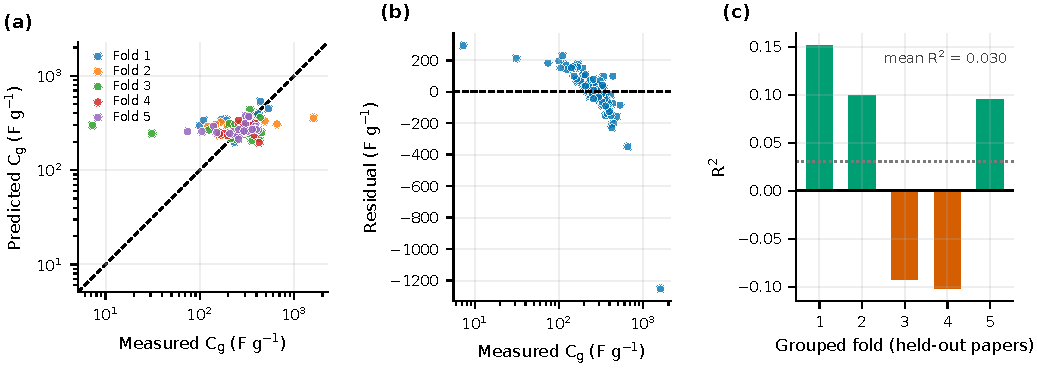
\includegraphics[width=\textwidth]{figures/fig02_grouped_prediction.pdf}
\caption{Paper-grouped cross-validation of the real-only model. (a) Measured versus
predicted capacitance for held-out papers, coloured by fold; the dashed line is parity.
(b) Residuals. (c) Per-fold $R^2$; the dotted line is the mean. Predictions regress towards
the corpus centre, which is the expected behaviour when each fold requires extrapolation to
an unobserved descriptor setting.}
\label{fig:grouped}\end{figure*}

\begin{table}[htbp]
\centering
\caption{Paper-grouped cross-validation of the real-only XGBoost model on the full descriptor set. MAE and RMSE in F\,g\textsuperscript{-1}. Rows from one publication never appear in both the training and test partition.}
\label{tab:grouped}
\footnotesize
\begin{tabular}{lrrrrrr}
\toprule
\textbf{Fold} & \textbf{$n_{\mathrm{train}}$} & \textbf{$n_{\mathrm{test}}$} & \textbf{Papers} & \textbf{$R^2$} & \textbf{MAE} & \textbf{RMSE} \\
\midrule
1 & 94 & 24 & 8 & 0.151 & 61.3 & 90.4 \\
2 & 94 & 24 & 8 & 0.099 & 134.7 & 278.7 \\
3 & 94 & 24 & 8 & -0.092 & 90.3 & 115.7 \\
4 & 95 & 23 & 8 & -0.102 & 52.4 & 73.9 \\
5 & 95 & 23 & 8 & 0.095 & 69.0 & 87.5 \\
\midrule \textbf{Mean} &  &  &  & \textbf{0.030} & \textbf{81.5} & \textbf{129.2} \\
SD &  &  &  & 0.119 & 32.8 & 84.9 \\
Median &  &  &  & 0.095 & 69.0 & 90.4 \\
Pooled &  &  &  & 0.081 & 81.9 & 150.8 \\
\bottomrule
\end{tabular}
\par\vspace{2pt}\begin{minipage}{\linewidth}\scriptsize ``Pooled'' scores every held-out prediction from every fold together, which avoids normalising by a near-zero within-fold target variance while keeping the grouped hold-out intact.\end{minipage}
\end{table}
\begin{table}[htbp]
\centering
\caption{One-way variance decomposition by source publication. $\eta^2$ is the share of total sum-of-squares lying between papers; ICC(1) is the corresponding intraclass correlation corrected for unequal group sizes.}
\label{tab:heterogeneity}
\footnotesize
\begin{tabular}{llrrrr}
\toprule
\textbf{Variable} & \textbf{Role} & \textbf{$n$} & \textbf{Papers} & \textbf{$\eta^2$} & \textbf{ICC(1)} \\
\midrule
current density A g & descriptor & 35 & 16 & 1.000 & 1.000 \\
pore diameter nm & descriptor & 4 & 4 & 1.000 & -- \\
h2so4 M & descriptor & 111 & 38 & 1.000 & 1.000 \\
ssa m2 g & descriptor & 35 & 17 & 0.989 & 0.980 \\
interlayer A & descriptor & 88 & 32 & 0.970 & 0.955 \\
electrode thickness um & descriptor & 54 & 20 & 0.969 & 0.955 \\
flake size um & descriptor & 11 & 6 & 0.727 & 0.493 \\
scan rate mV s & descriptor & 88 & 29 & 0.672 & 0.526 \\
target cap F g & target & 118 & 40 & 0.645 & 0.474 \\
mass loading mg cm2 & descriptor & 55 & 19 & 0.500 & 0.263 \\
\bottomrule
\end{tabular}
\par\vspace{2pt}\begin{minipage}{\linewidth}\scriptsize Values approaching unity mean a variable is essentially constant within a publication and varies only between publications, so holding out a whole paper requires the model to extrapolate rather than interpolate.\end{minipage}
\end{table}
